\section{Utilities}
While designing and implementing the computer, several supporting utilities were developed. The assembler (\texttt{bfasm}) is responsible for translating BF programs (text) into machine language (binary), the programmer and its software are used to write data to EEPROM chips and Mugen aids in having a more maintainable microcode definition. Each of these 3 utilities will be described in more detail below.

\subsection{Assembler: \texttt{bfasm}}
Even though the computer is designed to run BF natively, we can't just burn any text-file containing BF commands onto the program-ROM and expect it to execute them. Instead, each of these commands has to be translated into the binary opcodes that correspond to these commands. Table \ref{tab:opcodes} lists all the available commands and the values that map to these commands. As explained in Section \ref{sec:sequences}, there are a few non-BF that have been added.

\begin{table}[H]
  \centering
  \begin{tabular}{c|c}
    Command & Opcode \\ \hline
    \texttt{NOP} & 0x00 \\
    \texttt{+} & 0x01 \\
    \texttt{-} & 0x02 \\
    \texttt{<} & 0x03 \\
    \texttt{>} & 0x04 \\
    \texttt{,} & 0x05 \\
    \texttt{'} & 0x06 \\
    \texttt{.} & 0x07 \\
    \texttt{\detokenize{[}} & 0x08 \\
    \texttt{\detokenize{]}} & 0x09 \\
    \texttt{INIT} & 0x0d \\
    \texttt{HOME} & 0x0e \\
    \texttt{HLT}  & 0x0f 
  \end{tabular}
  \caption{Opcode values for each of the available commands.}
  \label{tab:opcodes}
\end{table}

\texttt{bfasm} performs pretty much a one-to-one transformation of the BF commands in the provided textfile into these values. It will add some preample commands to initialize the system and puts a \texttt{HLT} instruction at the end of the program to stop the computer when the program has finished (Figure \ref{fig:assembleoutput}). Part of the source-code is listed in the listing below; for the full source, refer to \url{https://github.com/jorenheit/bfcpu/blob/main/src/bfasm/bfasm.cc}.

\begin{figure}[H]
  \centering
  
\includegraphics[width=0.8\textwidth]{img/assembleroutput}
  \caption{Result of assembling a BF-file.}
  \label{fig:assembleoutput}
\end{figure}


\subsection{Programmer}

\begin{figure}[H]
  \centering
  \includegraphics[width=0.8\textwidth]{img/programmer}
  \caption{EEPROM chips were programmed using an Arduino Nano on a breadboard.}
  \label{fig:programmer}
\end{figure}

Given that there are four EEPROM chips embedded in the computer (one containing the program and three containing the microcode), we had to develop a toolkit for programming these. Specialized programmers can be pretty expensive and relatively hard to acquire, so an Arduino Nano was used to carry out that task. It waits for a serial connection and transfers incoming data byte per byte to the EEPROM chip. This serial connection is established by a Python script that accepts a binary blob and passes this on to the Arduino. The Python utility is called \texttt{bflash} (although it's not really BF-specific); its source and the Arduino sketch can be found at \url{https://github.com/jorenheit/bfcpu/tree/main/src/bflash}. A schematic for the programmer hardware (Figure \ref{fig:programmer}) is shown on the next page.

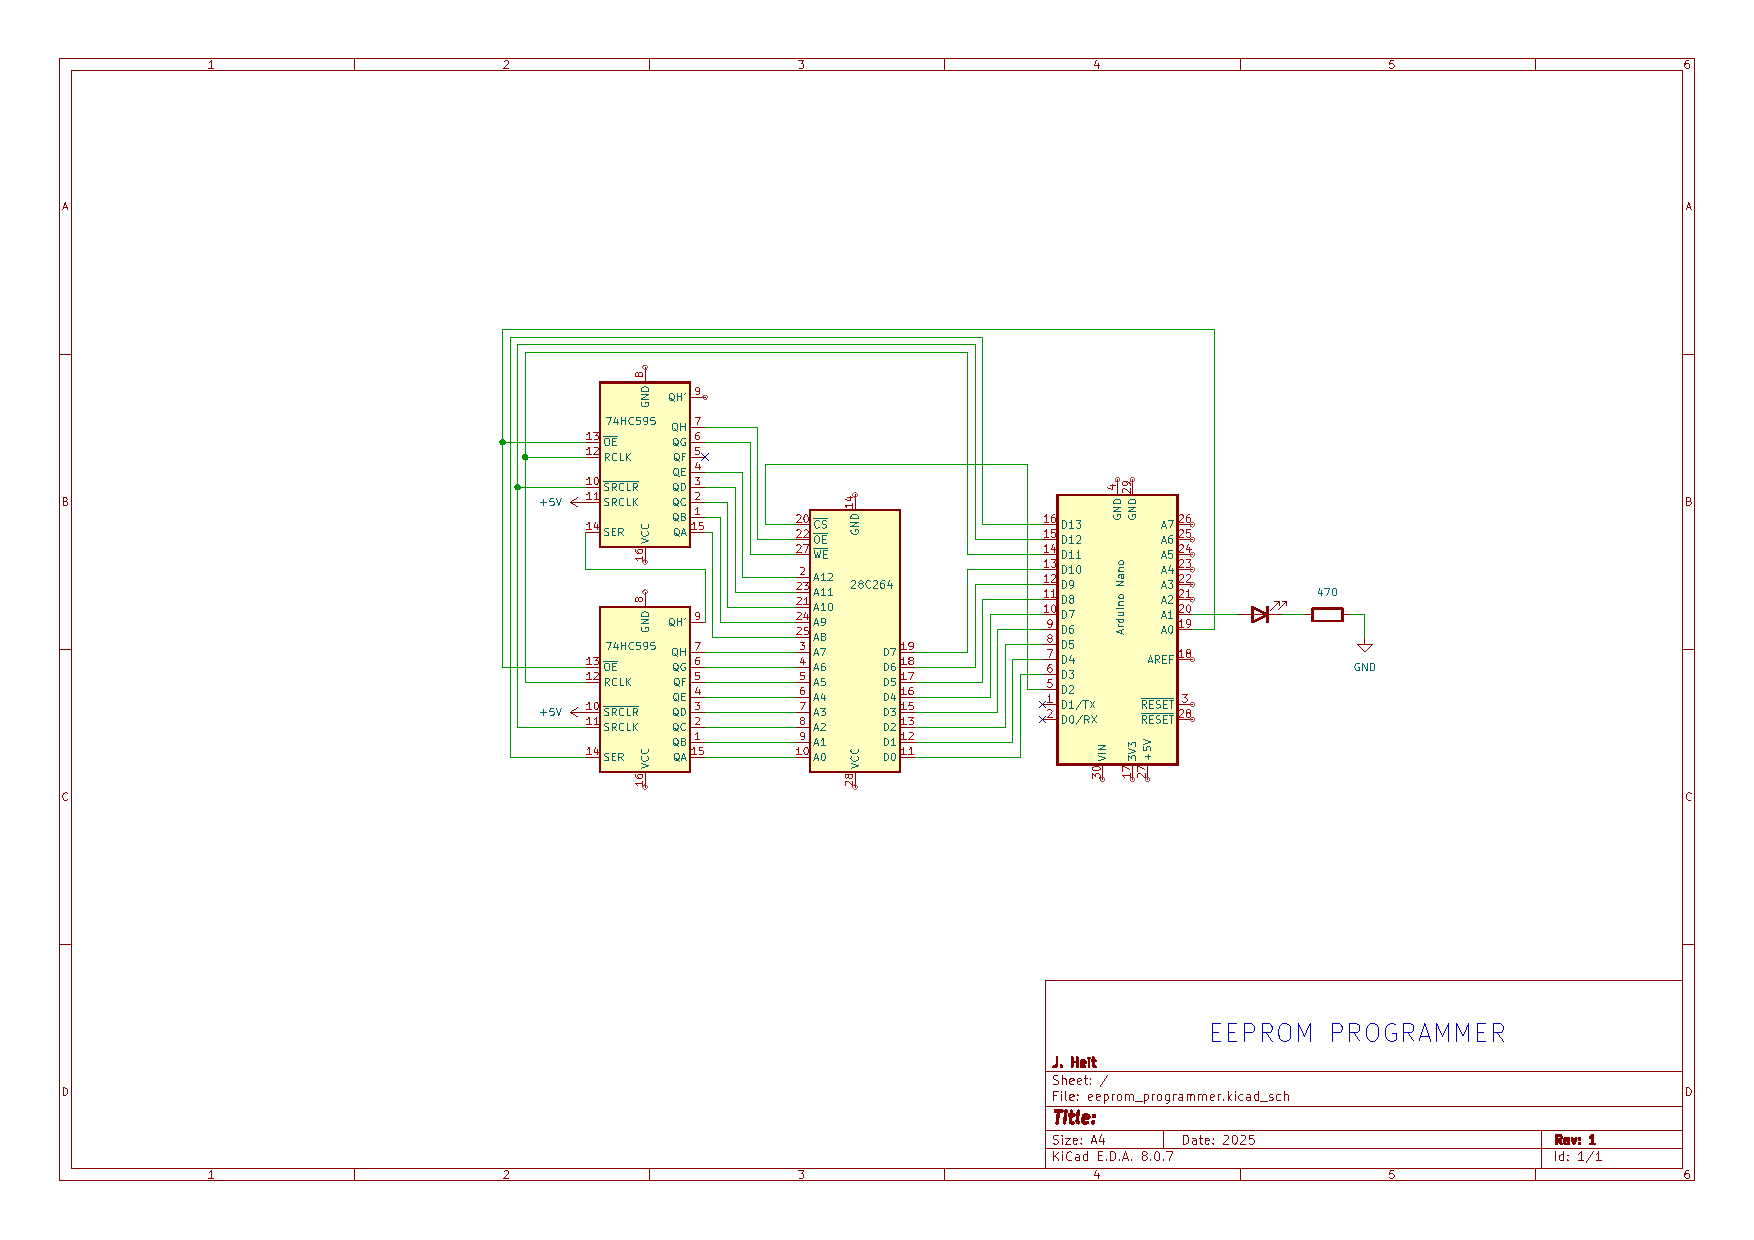
\includepdf[landscape=true]{schematics/eeprom_programmer.pdf}

\subsection{Microcode Generation (Mugen)}
Initially, the binary images that were burnt onto the microcode EEPROM chips were generated using a simple Octave/Matlab script. This meant that both the microcode and the logic to generate the images had to be expressed in this language. While this certainly worked (albeit a bit slow), we felt the need to develop a more general approach to generating microcode images. To satisfy this need, Mugen was developed. It takes a file in which the microcode can be expressed intuitively and generates the binary images from it. The Mugen project can be found in \url{https://github.com/jorenheit/mugen}. Section \ref{sec:implementation:cu} shows the Mugen specification file for this project. When this file is passed to Mugen, it shows the resulting memory layout. which corresponds to the layout as shown in the schematics of the Control Unit.

\begin{lstlisting}
$ mugen bfcpu.mu bfcpu.bin --layout
Successfully generated 3 images from bfcpu.mu: 
  ROM 0 : bfcpu.bin.0
  ROM 1 : bfcpu.bin.1
  ROM 2 : bfcpu.bin.2

[ROM 0, Segment 0] {
  0: HLT
  1: RS0
  2: RS1
  3: RS2
  4: INC
  5: DEC
  6: DPR
  7: EN_SP
}

[ROM 1, Segment 0] {
  0: OE_RAM
  1: WE_RAM
  2: EN_IN
  3: EN_OUT
  4: VE
  5: AE
  6: LD_FB
  7: LD_FA
}

[ROM 2, Segment 0] {
  0: EN_IP
  1: LD_IP
  2: EN_D
  3: LD_D
  4: CR
  5: ERR
  6: UNUSED
  7: UNUSED
}

[Address Layout] {
  0: CYCLE 0
  1: CYCLE 1
  2: CYCLE 2
  3: OPCODE 0
  4: OPCODE 1
  5: OPCODE 2
  6: OPCODE 3
  7: FLAG 0
  8: FLAG 1
  9: FLAG 2
  10: FLAG 3
  11: UNUSED
  12: UNUSED
}
\end{lstlisting}
